\section{Introduction}
\label{sec:Intro}

The rapid development of machine learning and 
especially deep learning has attracted the medical 
imaging community’s interest in applying these 
techniques to improve the accuracy of cancer 
screening. Breast cancer is the second leading 
cause of cancer deaths among U.S. women and 
screening mammography has been proved to reduce 
mortality
\cite{Oeffinger2015,Zhu2019}.
According to a study by the Breast 
Cancer Surveillance Consortium in 2009, the 
overall sensitivity of digital screening mammography 
in the U.S. is 84.4$\%$ and the overall specificity 
is 90.8$\%$
\cite{Jamieson2012}.
To help radiologists improve 
the predictive accuracy of screening mammography, 
computer-assisted detection and diagnosis (CAD) 
software have been developed and in clinical 
diagnosis since the 1990s. Unfortunately, data 
suggests that commercial CAD systems have not led 
to significant improvement in performance and 
progress has stagnated in the past decade
\cite{Girshick2015}.
With the remarkable success of deep learning in 
visual object recognition and detection, and many 
other domains have paid more attention to it
\cite{Lecun2015}.
There is much interest in developing deep 
learning tools to assist radiologists and improve 
the accuracy of screening mammography. 

Early detection of subclinical breast cancer on 
screening mammography is challenging as an image
classification task because the tumors themselves 
occupy only a small portion of the image of the
entire breast. For example, a full-field digital 
mammography (FFDM) image is typically 4000 × 3000
pixels while a cancerous region of interest (ROI) 
can be as small as 100 × 100 pixels. If ROI
annotations were widely available in mammography 
databases then established object detection and
classification methods such as the region-based 
convolutional neural network (R-CNN) and its
variants could be readily applied
\cite{Girshick2014,Girshick2015,Ren2017}.
However, approaches that require ROI annotations 
\cite{Dai2016}
often cannot be transferred to large mammography 
databases that lack ROI annotations, which are
laborious and costly to assemble. Indeed, few 
public mammography databases are annotated.
Yet, deep learning requires large training datasets 
to be most effective. Thus, it is essential to 
leverage both the few fully annotated datasets, as 
well as larger datasets labeled with only the 
cancer status of each image to improve the accuracy 
of breast cancer classification algorithms.

Pre-training is a promising method to address the 
training problem. For example 
\cite{Hinton2006,Li_2020},
used layer-wise pre-training to initialize the 
weight parameters of a deep belief net (DBN) with 
three hidden layers and then fine-tuned it for 
classification. They found that pre-training 
improved the training speed as well as the 
accuracy of handwritten digit recognition. Another 
popular training method is to first train a deep 
learning model on a large database such as the 
ImageNet 
\cite{Russakovsky2015,9112355}
and then fine-tune the model for another task. 
Although the specific task may not be related to 
the initial training dataset, the model’s weight 
parameters are already initialized for recognizing 
primitive features, such as edges, corners and 
textures, which can be readily used for a different 
task. This often saves training time and improves 
the model’s performance
\cite{He2016,Moreira2018}.

To take advantage of feature extraction ability of 
CNNs, recently researchers have proposed new 
mammography recognition methods. However, we think 
the ability to extratct the image features of 
deep CNNs could be better utilized. In this study, fusing 
different deep neural network models together to 
propose a fine-grained mammography image 
recognition approach via fusing multiple learned
features. Besides, utilizing the hash decoder
method to simplifying the classification 
calculation of complex high-dimensional 
feature vectors, and fusing the results of 
different classifier in the end. Our work can 
be summarized as follows:

1. Build a deep convolutional neural network based 
on well-performed network structures, and design a 
transfer learning strategy to improve the 
representation power of the extracted features.


2. To further utilize the feature representation 
ability of CNNs, we propose a method to fuse 
extracted features from multiple trained models 
with similar topological structure to
further improve the classification accuracy.

3. The strategy applied by hash learning in the 
deep network is cited to enhance the 
generalization ability of the model and solve the 
challenge of high-dimensional calculation 
in deep learning.

4. The designed feature fusion model is used in 
the feature extraction process of Faster RCNN, 
and a deep hash learning strategy is introduced 
in the classification stage.

The rest of this paper is organized as follows. 
Section~\ref{sec:Meth} 
details of the network structure and the proposed 
method. 
Section~\ref{sec:Data} 
elaborates the dataset used in our work.
Section~\ref{sec:Exp} 
demonstrates the experiment results and gives 
discussion. 
Section~\ref{sec:Conc} 
makes the conclusion and future work are provided 
in the end.

\begin{figure*}[!ht]
    \centering
    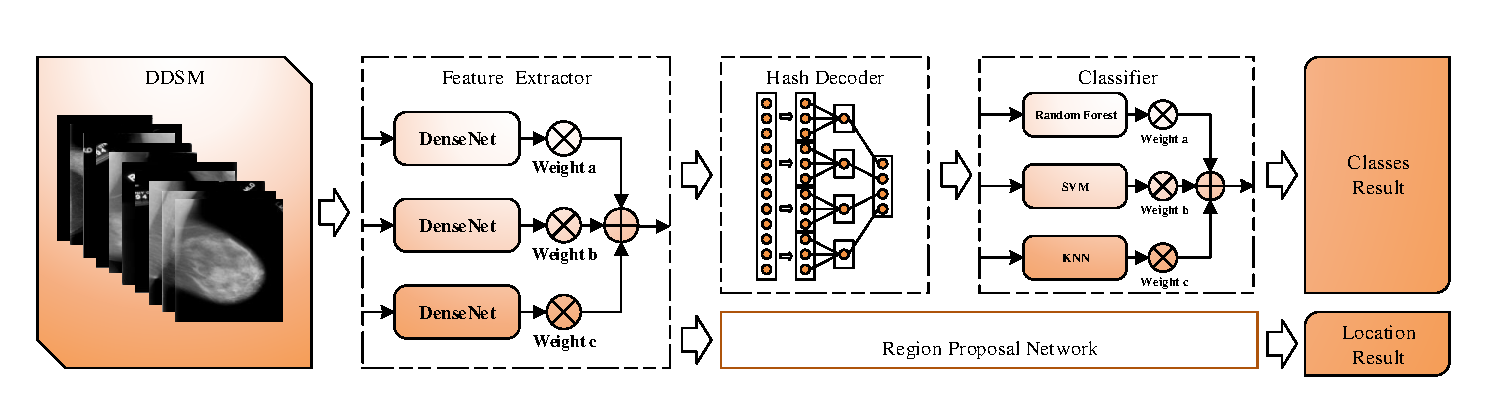
\includegraphics[
        width=1.0\textwidth,
        keepaspectratio
    ]{NetStruct.pdf}
    \caption{Overview of the proposed approach.}
    \label{fig:netStruct}
\end{figure*}
